\documentclass[12pt,a4paper]{report}

\usepackage[utf8]{inputenc}
\usepackage[T5]{fontenc}
\usepackage[vietnamese]{babel}
\usepackage{graphicx}
\usepackage{amsmath}
\usepackage{amssymb}
\usepackage{algorithm}
\usepackage{algpseudocode}

\usepackage{geometry}
\geometry{a4paper, left=3cm, right=2cm, top=2cm, bottom=2cm}
\usepackage{hyperref}
\usepackage{setspace}
\usepackage{titlesec}
\usepackage{tocloft}
\usepackage{fancyhdr}
\usepackage{tikz}
\usetikzlibrary{calc, positioning, arrows.meta}

\pagestyle{fancy}
\fancyhf{}
\fancyhead[L]{Khóa luận chuyên ngành Khoa học dữ liệu}
\renewcommand{\headrulewidth}{0.4pt}
\fancyfoot[C]{\thepage}

% Định nghĩa viền đôi cho trang bìa
\newcommand{\drawborder}{
    \begin{tikzpicture}[remember picture, overlay]
        \draw[line width=2pt] ($(current page.south west) + (2cm,2cm)$) rectangle ($(current page.north east) - (1.5cm,2cm)$);
        \draw[line width=0.5pt] ($(current page.south west) + (2.1cm,2.1cm)$) rectangle ($(current page.north east) - (1.6cm,2.1cm)$);
    \end{tikzpicture}
}

\linespread{1.5} % Khoảng cách dòng chuẩn theo mẫu
\setlength{\parskip}{4.5pt} % Khoảng cách giữa các đoạn văn

\begin{document}

% ------------------------- TRANG BÌA NGOÀI -------------------------
\begin{titlepage}
    \thispagestyle{empty}
    \drawborder
    \begin{center}
        \textbf{\large ĐẠI HỌC QUỐC GIA TP. HỒ CHÍ MINH} \\
        \textbf{\large TRƯỜNG ĐẠI HỌC KHOA HỌC TỰ NHIÊN} \\
        \textbf{\large KHOA TOÁN - TIN HỌC} \\
        \vspace{2cm}
        
        % Chèn logo của trường
        
\includegraphics[width=6cm]{logo khtn.png} \\
        \vspace{2.5cm}
        
        \textbf{\Large Khóa luận tốt nghiệp} \\
        \vspace{2cm}
        
        \textbf{\Large CẢI THIỆN THUẬT TOÁN SELF-DISTILLATION POLICY OPTIMIZATION \\[0.2cm] CHO MÔ HÌNH NGÔN NGỮ LỚN \\[0.2cm] TRONG BÀI TOÁN SUY LUẬN TOÁN HỌC} \\
        
        \vfill
        \large
        \textit{Tp. Hồ Chí Minh - 2026}
    \end{center}
\end{titlepage}

% ------------------------- TRANG BÌA TRONG -------------------------
\begin{titlepage}
    \thispagestyle{empty}
    \drawborder
    \begin{center}
        \textbf{\large ĐẠI HỌC QUỐC GIA TP. HỒ CHÍ MINH} \\
        \textbf{\large TRƯỜNG ĐẠI HỌC KHOA HỌC TỰ NHIÊN} \\
        \textbf{\large KHOA TOÁN - TIN HỌC} \\
        \vspace{1cm}
        
        % Chèn logo của trường
        
\includegraphics[width=6cm]{logo khtn.png} \\
        \vspace{1cm}
        
        \textbf{\Large Khóa luận tốt nghiệp} \\
        \vspace{1cm}
        
        \textbf{\Large CẢI THIỆN THUẬT TOÁN SELF-DISTILLATION POLICY OPTIMIZATION \\[0.2cm] CHO MÔ HÌNH NGÔN NGỮ LỚN \\[0.2cm] TRONG BÀI TOÁN SUY LUẬN TOÁN HỌC} \\
        \vspace{1cm}
        
        \large CHUYÊN NGÀNH KHOA HỌC DỮ LIỆU \\
        \vspace{1cm}
        
        \begin{tabular}{@{}ll@{}}
            \textbf{\large Giảng viên hướng dẫn:} & \large TS. NGÔ MINH MẪN \\[0.5cm]
            \textbf{\large Sinh viên thực hiện:} & \large TÔ GIA BẢO - 22280006 \\
            & \large PHAN VĂN HOÀNG - 22280033
        \end{tabular}
        
        \vfill
        \large
        \textit{Tp. Hồ Chí Minh - 2026}
    \end{center}
\end{titlepage}

% ------------------------- LỜI CẢM ƠN -------------------------
\chapter*{LỜI CẢM ƠN}
\addcontentsline{toc}{chapter}{LỜI CẢM ƠN}
Lời đầu tiên, chúng em xin gửi lời cảm ơn chân thành đến Khoa Toán - Tin học và Trường Đại học Khoa học Tự nhiên, ĐHQG-HCM đã tạo điều kiện cho chúng em được học tập và rèn luyện trong môi trường giáo dục chất lượng cao, giúp chúng em có cơ hội thực hiện khóa luận tốt nghiệp này.

Chúng em đặc biệt biết ơn TS. Ngô Minh Mẫn, người đã tận tâm hướng dẫn, chỉ bảo chúng em trong suốt quá trình thực hiện đề tài. Nhờ sự nhiệt tình và tận tâm của thầy, chúng em đã được trang bị những kiến thức và kỹ năng cần thiết để hoàn thành khóa luận tốt nghiệp một cách tốt đẹp nhất.

Chúng em cũng xin gửi lời tri ân đến gia đình, đặc biệt là ba mẹ - những người đã luôn yêu thương, động viên và tạo điều kiện tốt nhất cho chúng em học tập và theo đuổi đam mê. Nhờ sự ủng hộ tinh thần to lớn của gia đình, chúng em đã có thêm động lực.

% ------------------------- LỜI MỞ ĐẦU -------------------------
\chapter*{LỜI MỞ ĐẦU}
\addcontentsline{toc}{chapter}{LỜI MỞ ĐẦU}
Trong những năm gần đây, các Mô hình Ngôn ngữ Lớn (LLMs) đã đạt được những bước tiến vượt bậc, thể hiện khả năng xuất sắc trong nhiều lĩnh vực, đặc biệt là các tác vụ đòi hỏi tư duy logic như suy luận toán học. Tuy nhiên, để các mô hình này thực sự làm chủ được các bài toán nhiều bước, quá trình tinh chỉnh (post-training) bằng học tăng cường đóng vai trò vô cùng quan trọng. 

Các phương pháp học tăng cường truyền thống, chẳng hạn như GRPO, thường chỉ tối ưu hóa dựa trên một phần thưởng vô hướng duy nhất ở cuối chuỗi sinh văn bản. Đối với các bài toán toán học phức tạp, điều này tạo ra "nút thắt phân bổ tín nhiệm" nghiêm trọng, vì mô hình không thể nhận biết chính xác bước lập luận nào trong toàn bộ chuỗi tư duy là sai lầm. Gần đây, thuật toán Self-Distillation Policy Optimization (SDPO) đã ra đời nhằm biến các phản hồi văn bản thành tín hiệu tự sửa lỗi. Dù mang lại hiệu quả đột phá, SDPO khi áp dụng vào suy luận toán học vẫn đối mặt với bài toán hóc búa về độ tin cậy của quá trình tự học và chi phí tính toán cao.

Xuất phát từ thực tiễn trên, đề tài: \textbf{“Cải thiện thuật toán Self-Distillation Policy Optimization cho mô hình ngôn ngữ lớn trong bài toán suy luận toán học”} được lựa chọn để nghiên cứu. Khóa luận tập trung triển khai cơ chế Cổng độ tin cậy (Reliability Gate) nhằm lọc tín hiệu nhiễu trong quá trình tự chưng cất; hệ thống được xây dựng và huấn luyện trên dòng mô hình Qwen3 thông qua nền tảng mã nguồn mở Verl. 

Kết quả thực nghiệm cho thấy cơ chế cải tiến đã giúp mô hình chọn lọc hiệu quả các chuỗi tư duy chất lượng và tránh việc học theo các suy luận sai lệch (misleading reasoning). Hơn nữa, thông qua cơ chế thực thi thưa (sparse target execution), thuật toán loại bỏ hoàn toàn việc tính toán hàm mất mát cho các mẫu rác, qua đó tối ưu hóa mạnh mẽ tài nguyên phần cứng. Việc áp dụng thành công SDPO cải tiến không chỉ nâng cao tính ổn định, tiết kiệm chi phí huấn luyện mà còn cải thiện rõ rệt độ chính xác của LLMs khi giải quyết các bài toán suy luận phức tạp.

% ------------------------- DANH SÁCH TỪ VIẾT TẮT -------------------------
\chapter*{DANH SÁCH TỪ VIẾT TẮT}
\addcontentsline{toc}{chapter}{DANH SÁCH TỪ VIẾT TẮT}
(Phần nội dung danh sách từ viết tắt - Sinh viên tự bổ sung sau)

% ------------------------- DANH MỤC -------------------------
\tableofcontents
\listoffigures
\listoftables

\clearpage
\pagenumbering{arabic} % Đánh số trang 1, 2, 3... bắt đầu từ đây

% ------------------------- CHƯƠNG 1 -------------------------
\chapter{GIỚI THIỆU ĐỀ TÀI}

\section{Bối cảnh của đề tài}
Sự bùng nổ của các Mô hình Ngôn ngữ Lớn (LLMs) như GPT-4 hay Qwen đã mở ra tiềm năng tự động hóa các tác vụ đòi hỏi tư duy logic phức tạp, tiêu biểu là suy luận toán học. Khác với các tác vụ xử lý ngôn ngữ tự nhiên cơ bản, toán học yêu cầu mô hình phải lập luận qua nhiều bước (Chain-of-Thought) với tính chính xác tuyệt đối. 

Tuy nhiên, trí thông minh này không chỉ đến từ việc huấn luyện trước (pre-training) trên lượng dữ liệu khổng lồ. Để LLMs thực sự làm chủ cách giải bài toán theo từng bước lô-gic, quá trình tinh chỉnh (post-training) bằng Học tăng cường (Reinforcement Learning - RL) đóng vai trò quyết định. RL giúp căn chỉnh phản hồi của mô hình theo đúng lô-gic yêu cầu, là chìa khóa để khai mở tiềm năng giải toán của LLMs.

\section{Lý do thực hiện đề tài, vấn đề nghiên cứu}
Mặc dù đóng vai trò then chốt, các thuật toán RL truyền thống (tiêu biểu như GRPO) lại có giới hạn bản chất trong miền suy luận toán học.

\textbf{Thứ nhất, nút thắt phân bổ tín nhiệm.} RL truyền thống thường đánh giá mô hình bằng một điểm số vô hướng duy nhất ở cuối chuỗi sinh (ví dụ: +1 nếu đúng, 0 nếu sai). Khi bài toán cần hàng chục bước giải, việc chỉ cung cấp một điểm số tạo ra "nút thắt phân bổ tín nhiệm" nghiêm trọng. Mô hình không thể nhận biết chính xác bước lập luận nào trong chuỗi là sai lầm.

\textbf{Thứ hai, lãng phí phản hồi văn bản.} Các môi trường kiểm chứng thực tế không chỉ trả về đúng/sai mà thường cung cấp lỗi hoặc giải thích chi tiết. Các phương pháp RL truyền thống hoàn toàn bỏ qua nguồn dữ liệu phong phú này. 

Để khắc phục, Tối ưu hóa Chính sách Tự chưng cất (SDPO) đã được đề xuất. SDPO trực tiếp sử dụng LLM làm "người thầy". Khi giải sai, mô hình nhận phản hồi văn bản, tự sinh lời giải mới tốt hơn, rồi dùng nó để tự chưng cất và cập nhật chính sách.

\textbf{Vấn đề nghiên cứu đặt ra:} Tuy mang tính đột phá, SDPO đối mặt với hai thách thức chí mạng khi áp dụng vào miền Toán học:
\begin{itemize}
    \item \textit{Mô phỏng suy luận sai lệch (Noisy Imitation):} SDPO nguyên bản giả định mọi mục tiêu chưng cất từ phản hồi đều có ích. Tuy nhiên, trong toán học, một lời giải sai vẫn có thể là một chuỗi suy luận dài, trôi chảy nhưng chứa các bước lập luận sai lầm. Việc "bắt chước" mù quáng các mục tiêu này sẽ làm củng cố các tư duy sai lệch của mô hình.
    \item \textit{Lãng phí tài nguyên tính toán (Compute Waste):} Đặc thù của thuật toán SDPO là bổ sung thêm nhánh tính toán đắt đỏ (teacher inputs, teacher logits) lên trên quá trình Rollout sinh dữ liệu. Việc thực hiện các tính toán khổng lồ này trên cả những chuỗi lập luận vô nghĩa hoặc bị cắt xén gây ra sự lãng phí nghiêm trọng về thời gian và bộ nhớ GPU.
\end{itemize}
Do đó, việc cải tiến SDPO để vừa lọc nhiễu, vừa giảm thiểu chi phí tính toán là một yêu cầu cấp thiết.

\section{Mục tiêu nghiên cứu}
\textbf{Mục tiêu tổng quát:} Cải tiến thuật toán SDPO nhằm nâng cao độ tin cậy và khắc phục hiện tượng suy giảm hiệu suất, gia tăng năng lực giải quyết bài toán suy luận toán học của LLMs.

\textbf{Mục tiêu cụ thể:}
\begin{itemize}
    \item Tích hợp cơ chế Cổng độ tin cậy (Reliability Gate) để đánh giá trọng số tín nhiệm, chỉ lựa chọn các mục tiêu đã được xác minh hoặc có phản hồi an toàn làm dữ liệu chưng cất.
    \item Cấu hình quy trình huấn luyện phân tán, áp dụng cơ chế thực thi thưa (Sparse Target Execution) và điều tiết ngân sách lô (Batch Budget) nhằm giảm đáng kể lãng phí tài nguyên tính toán (Compute Waste).
    \item Huấn luyện các phiên bản thuật toán (Base RL, Vanilla SDPO, Reliability-Gated SDPO) trên nền tảng Verl với mô hình Qwen3, so sánh hiệu suất và thời gian thực thi trên tập dữ liệu DAPO-Math.
\end{itemize}

\section{Phương pháp nghiên cứu}
Khóa luận sử dụng kết hợp các phương pháp sau:

\textbf{1. Nghiên cứu tài liệu:} Khảo sát, phân tích các nghiên cứu về LLM, RLHF, kỹ thuật Chain-of-Thought và thuật toán SDPO.

\textbf{2. Nghiên cứu thực nghiệm và đánh giá:} 
Mô hình được thiết lập huấn luyện phân tán trên cụm GPU bằng framework mã nguồn mở Verl/Ray. Quá trình đánh giá được thực hiện thông qua việc so sánh SDPO với Baseline (GRPO) dựa trên các nhóm độ đo (metrics) chuẩn:
\begin{itemize}
    \item \textbf{Độ chính xác (Validation Accuracy):} Đánh giá tỷ lệ giải toán đúng trên tập dữ liệu kiểm thử được trích xuất (held-out subset).
    \item \textbf{Định dạng và Chiều dài (Format \& Truncation):} Tỷ lệ đầu ra sai định dạng hoặc bị cắt xén do vượt giới hạn token, kết hợp đánh giá độ dài trung bình của câu trả lời.
    \item \textbf{Hiệu suất hệ thống (Throughput \& Execution Time):} Thông lượng đào tạo tổng thể (số token/giây) và thời gian thực thi chi tiết cho các pha sinh dữ liệu (Rollout), tính toán Teacher Logits và cập nhật Actor.
    \item \textbf{Chỉ số Cổng độ tin cậy (SDPO Metrics):} Đo lường tỷ lệ các mẫu được chọn lọc làm mục tiêu SDPO so với lượng ngân sách cho phép, và số phần trăm tính toán (Compute Token Fraction) tiết kiệm được.
\end{itemize}

\section{Kết cấu của đề tài và giới hạn đề tài}

\textbf{Giới hạn đề tài:} 
\begin{itemize}
    \item \textit{Miền ứng dụng:} Chỉ tập trung vào suy luận toán học nhiều bước.
    \item \textit{Mô hình nền tảng:} Sử dụng Qwen3 để đảm bảo khả năng tính toán trên phần cứng giới hạn.
    \item \textit{Bộ dữ liệu:} Thử nghiệm trên tập dữ liệu chuẩn DAPO-Math.
\end{itemize}

\textbf{Kết cấu của đề tài:}
Ngoài phần mở đầu và danh mục, khóa luận gồm 5 chương:
\begin{itemize}
    \item \textbf{Chương 1: Giới thiệu đề tài.} Bối cảnh, lý do, mục tiêu, phương pháp và giới hạn nghiên cứu.
    \item \textbf{Chương 2: Cơ sở lý thuyết.} Kiến thức nền tảng về LLM, Học tăng cường, SDPO và Verl/vLLM.
    \item \textbf{Chương 3: Phương pháp và giải pháp đề xuất.} Hạn chế của SDPO nguyên bản và kiến trúc thuật toán cải tiến (Reliability Gate).
    \item \textbf{Chương 4: Thực nghiệm và đánh giá.} Môi trường thực nghiệm, cấu hình huấn luyện và phân tích kết quả định lượng.
    \item \textbf{Chương 5: Kết luận và hướng phát triển.} Tóm tắt đóng góp, hạn chế và hướng phát triển tương lai.
\end{itemize}

% ------------------------- CHƯƠNG 2 -------------------------
\chapter{CƠ SỞ LÝ THUYẾT VÀ CÔNG NGHỆ TƯƠNG QUAN}

\section{Tổng quan về Học tăng cường (Reinforcement Learning)}
Học tăng cường (Reinforcement Learning - RL) là một nhánh của học máy, trong đó một \textit{tác tử (agent)} học cách đưa ra các quyết định thông qua việc tương tác thử-sai với một \textit{môi trường (environment)} nhằm tối đa hóa phần thưởng tích lũy (cumulative reward) nhận được. 

Về mặt toán học, bài toán học tăng cường được mô hình hóa thành một Quá trình ra quyết định Markov (Markov Decision Process - MDP) được định nghĩa bởi bộ 5 thành phần $(\mathcal{S}, \mathcal{A}, \mathcal{P}, \mathcal{R}, \gamma)$, trong đó:
\begin{itemize}
    \item $\mathcal{S}$ là tập hợp các \textit{trạng thái (states)} của môi trường. Trạng thái tại thời điểm $t$ ký hiệu là $S_t$.
    \item $\mathcal{A}$ là tập hợp các \textit{hành động (actions)} mà tác tử có thể thực hiện. Hành động tại thời điểm $t$ ký hiệu là $A_t$.
    \item $\mathcal{P}(S_{t+1}|S_t, A_t)$ là xác suất chuyển đổi, tức xác suất môi trường chuyển sang trạng thái tiếp theo $S_{t+1}$ khi tác tử thực hiện hành động $A_t$ ở trạng thái hiện tại $S_t$.
    \item $\mathcal{R}(S_t, A_t, S_{t+1})$ là hàm \textit{phần thưởng (reward)} mang tính phản hồi, trả về giá trị vô hướng $R_{t+1}$ khi tác tử thực hiện hành động $A_t$.
    \item $\gamma \in [0, 1]$ là hệ số chiết khấu (discount factor), định lượng tầm quan trọng của các phần thưởng trong tương lai so với phần thưởng hiện tại.
\end{itemize}

Sự tương tác liên tục và tuần tự này giữa tác tử và môi trường được trực quan hóa chi tiết trong Hình \ref{fig:mdp_model}.

\begin{figure}[h!]
    \centering
    \vspace{0.5cm}
    \begin{tikzpicture}[
        box/.style={draw, rectangle, minimum width=3.5cm, minimum height=1.2cm, align=center, thick, rounded corners=5pt, fill=blue!5},
        arrow/.style={->, >=stealth, thick, rounded corners=5pt}
    ]
        % Nodes
        \node[box] (agent) at (0, 3) {\textbf{Tác tử} \\ (Agent)};
        \node[box] (env) at (0, 0) {\textbf{Môi trường} \\ (Environment)};
        
        % Right side: Action
        \draw[arrow] (agent.0) -- +(1.5,0) |- node[pos=0.25, right, align=left] {Hành động\\$A_t$} (env.0);
        
        % Left side coordinates
        \coordinate (env_R) at ([yshift=3mm]env.180);
        \coordinate (env_S) at ([yshift=-3mm]env.180);
        \coordinate (agent_R) at ([yshift=-3mm]agent.180);
        \coordinate (agent_S) at ([yshift=3mm]agent.180);
        
        % Coordinates for dashed line intersection
        \coordinate (dash_R) at ([xshift=-1.5cm]env_R);
        \coordinate (dash_S) at ([xshift=-1.5cm]env_S);
        
        % Environment output to dashed line (with arrowheads ON the dashed line)
        % Place R_{t+1} above the top line, S_{t+1} below the bottom line to prevent overlap
        \draw[arrow] (env_R) -- node[above] {$R_{t+1}$} (dash_R);
        \draw[arrow] (env_S) -- node[below] {$S_{t+1}$} (dash_S);
        
        % Vertical dashed line (time step separator)
        \draw[dashed, thick] ([xshift=-1.5cm, yshift=-7mm]env.180) -- ([xshift=-1.5cm, yshift=7mm]env.180);
        
        % Dashed line to Agent
        % Inner loop (Reward) - goes left by 1cm
        \draw[arrow] (dash_R) -- +(-1cm, 0) |- node[pos=0.25, right, align=left] {Phần thưởng\\$R_t$} (agent_R);
        
        % Outer loop (State) - goes left by 1.6cm (so the two vertical lines are 0.6cm apart)
        \draw[arrow] (dash_S) -- +(-1.6cm, 0) |- node[pos=0.25, left, align=right] {Trạng thái\\$S_t$} (agent_S);

    \end{tikzpicture}
    \vspace{0.5cm}
    \caption{Mô hình hóa Quá trình ra quyết định Markov (MDP)}
    \label{fig:mdp_model}
\end{figure}

\subsection{Chính sách và Chính sách tối ưu (Policy \& Optimal Policy)}

Để tương tác với môi trường và đưa ra quyết định, tác tử tuân theo một \textit{chính sách (policy)} $\pi$. Có thể hiểu chính sách là một bộ quy tắc, chiến lược cốt lõi của tác tử để quyết định xem nó nên thực hiện hành động nào tiếp theo khi đang ở một trạng thái cụ thể. Trong lý thuyết MDP, chính sách được chia làm hai loại chính:
\begin{itemize}
    \item \textbf{Chính sách xác định (Deterministic Policy):} Ký hiệu là $A_t = \pi(S_t)$. Với mỗi trạng thái $S_t$, tác tử luôn luôn chọn đúng một hành động duy nhất $A_t$.
    \item \textbf{Chính sách ngẫu nhiên (Stochastic Policy):} Ký hiệu là $\pi(A_t|S_t) = \mathbb{P}(A_t|S_t)$. Ở đây, chính sách được biểu diễn dưới dạng một phân phối xác suất. Tác tử sẽ lựa chọn hành động $A_t$ thông qua việc lấy mẫu từ phân phối này tại trạng thái $S_t$. Trong bối cảnh của các Mô hình Ngôn ngữ Lớn (LLMs), các mô hình hoạt động theo chính sách ngẫu nhiên; tại mỗi bước, LLM sinh ra một từ (token) tiếp theo dựa trên phân phối xác suất dự đoán qua toàn bộ không gian từ vựng.
\end{itemize}

Mục tiêu cốt lõi và tối thượng của bất kỳ bài toán học tăng cường nào là tìm ra một \textit{chính sách tối ưu (optimal policy)}, ký hiệu là $\pi^*$. Một chính sách được coi là tối ưu nếu và chỉ nếu kỳ vọng tổng phần thưởng tích lũy (expected cumulative reward) mà tác tử thu về khi tuân theo chính sách đó lớn hơn hoặc bằng bất kỳ chính sách nào khác, trên mọi trạng thái có thể có của môi trường. Về mặt toán học, chính sách tối ưu được biểu diễn bằng bài toán tối đa hóa:
\begin{equation}
    \pi^* = \arg\max_\pi \mathbb{E}_{\tau \sim \pi} \left[ \sum_{t=0}^T \gamma^t R_{t+1} \right]
\end{equation}
Trong đó, $\tau$ (trajectory) là chuỗi các trạng thái và hành động mà tác tử thực hiện từ đầu đến cuối.

\subsection{Hàm giá trị (Value Function)}
Hàm giá trị $V^\pi(s)$ là một thành phần không thể thiếu trong MDP, biểu diễn kỳ vọng tổng phần thưởng tích lũy mà tác tử sẽ nhận được bắt đầu từ trạng thái $s$ và làm theo chính sách $\pi$ cho đến khi kết thúc quá trình:
\begin{equation}
    V^\pi(s) = \mathbb{E}_\pi \left[ \sum_{k=0}^\infty \gamma^k R_{t+k+1} \middle| S_t = s \right]
\end{equation}
Hàm giá trị giúp tác tử đánh giá xem việc ở tại một trạng thái cụ thể là "tốt" hay "xấu" về mặt dài hạn, từ đó định hướng cho việc cập nhật chính sách $\pi$ dần tiến tới mức tối ưu $\pi^*$.

Về mặt tổng thể, MDP cung cấp một khung toán học chặt chẽ để mô hình hóa quá trình tương tác tuần tự. Trong đó, trạng thái ($S_t$) biểu diễn tình huống hiện tại của hệ thống, hành động ($A_t$) đại diện cho quyết định được đưa ra, phần thưởng ($R_{t+1}$) là tín hiệu định lượng đánh giá chất lượng của quyết định đó, và chính sách ($\pi$) đóng vai trò là hàm ánh xạ chiến lược. Quá trình huấn luyện mô hình học tăng cường chính là quá trình tối ưu hóa hàm ánh xạ này để hội tụ về chính sách tối ưu ($\pi^*$).

\section{Mô hình Ngôn ngữ Lớn và Suy luận Toán học}
Các Mô hình Ngôn ngữ Lớn (LLMs) được xây dựng dựa trên kiến trúc Transformer, cho phép xử lý và sinh văn bản tự nhiên thông qua việc dự đoán token tiếp theo một cách tự hồi quy (autoregressive). Gọi $x$ là câu hỏi đầu vào và $y = (y_1, y_2, \dots, y_T)$ là chuỗi câu trả lời, phân phối xác suất của mô hình $\pi_\theta$ được định nghĩa là:
\begin{equation}
    \pi_\theta(y|x) = \prod_{t=1}^T \pi_\theta(y_t | x, y_{<t})
\end{equation}
Trong miền suy luận toán học, quá trình sinh văn bản này được mô hình hóa như một dạng lập luận tự điều chỉnh (\textit{self-Bayesian reasoning}). Ở đó, mỗi bước giải (Chain-of-Thought) phụ thuộc vào cả bài toán gốc và các bước lập luận trước đó, cho phép mô hình liên tục cập nhật niềm tin (belief) của nó về các giả thuyết trung gian. Khác với các tác vụ ngôn ngữ thông thường, toán học đòi hỏi tính chính xác tuyệt đối và khả năng duy trì tính logic qua nhiều bước.

\section{Học tăng cường: Từ GRPO đến SDPO}

\subsection{Học tăng cường với phần thưởng kiểm chứng (RLVR) và Phản hồi phong phú (RLRF)}

Khái niệm Học tăng cường với Phần thưởng Kiểm chứng (Reinforcement Learning from Verifiable Rewards - RLVR) \cite{kyars2026rlvr} nổi lên như một xu hướng cốt lõi để nâng cao năng lực suy luận toán học của các Mô hình Ngôn ngữ Lớn. Khác với RLHF (dựa vào con người) hay RLAIF (dựa vào mô hình giám khảo), RLVR tận dụng tín hiệu phần thưởng từ những tác vụ có khả năng tự kiểm chứng (checkable tasks). Cốt lõi của RLVR nằm ở \textit{bộ kiểm chứng (verifier)} — cơ chế tự động trích xuất đáp án (ví dụ: chuỗi nằm trong thẻ \texttt{<answer>}) và đánh giá tính tương đương với đáp án chuẩn một cách khách quan.

Tuy nhiên, phần lớn các cách tiếp cận hiện tại của RLVR đều hoạt động dựa trên thiết lập \textit{phần thưởng kết quả vô hướng (Scalar Outcome Reward)}: cho một câu hỏi $x$, mô hình sinh ra một câu trả lời $y \sim \pi_\theta(\cdot|x)$ và nhận được một phần thưởng vô hướng $r \in \mathbb{R}$, thường là giá trị nhị phân (ví dụ: đúng/sai trong toán học, pass/fail đối với test cases trong lập trình). Việc chỉ dựa vào một con số duy nhất ở cuối cùng này tạo ra một \textbf{nút thắt thông tin (information bottleneck)}. Điểm số $r$ sau đó bị phân bổ đồng đều cho mọi token, dẫn đến \textbf{bài toán phân bổ tín nhiệm (credit assignment problem)}. Một chuỗi lập luận có bước logic sai nhưng vô tình ra đáp án đúng sẽ khiến mô hình được cộng điểm cho những suy luận sai lầm đó. Ngược lại, một chuỗi đúng 90\% nhưng tính sai ở bước cuối cùng lại bị phạt toàn bộ.

Để khắc phục, \textit{phần thưởng quá trình (Process Reward)} được đề xuất nhằm đánh giá từng bước trung gian. Dù vậy, việc huấn luyện một Mô hình Phần thưởng Quá trình (PRM) đòi hỏi chi phí gán nhãn khổng lồ. Bên cạnh đó, ở các thuật toán RL truyền thống, việc đánh giá hàm giá trị (value function) cho từng trạng thái trung gian đòi hỏi duy trì một mạng nơ-ron phụ trợ riêng biệt (value network) có kích thước tương đương mô hình chính, làm nhân đôi chi phí bộ nhớ trong quá trình huấn luyện.

Để vượt qua những rào cản này, khái niệm \textbf{Học tăng cường với Phản hồi Phong phú (Reinforcement Learning with Rich Feedback - RLRF)} được đề xuất. Thay vì giới hạn ở một tín hiệu vô hướng đơn nhất, RLRF tận dụng các luồng \textit{phản hồi văn bản (textual feedback)} được mã hóa dưới dạng token từ môi trường (như thông báo lỗi biên dịch hoặc giải thích chi tiết từ các trình đánh giá). Các phản hồi này không chỉ cung cấp kết quả nhị phân (đúng/sai) mà còn biểu đạt nguyên nhân dẫn đến sự thất bại, từ đó cung cấp ngữ cảnh để mô hình tự điều chỉnh hành vi. Sự khác biệt mang tính bước ngoặt giữa phương pháp phần thưởng vô hướng (RLVR) và phản hồi phong phú (RLRF) được minh họa rõ nét trong Hình \ref{fig:rlvr_vs_rlrf}.

\begin{figure}[h!]
    \centering
    \begin{tikzpicture}[
        agent_env/.style={draw, rectangle, rounded corners=3pt, minimum width=2cm, minimum height=0.6cm, fill=gray!10, font=\small\bfseries},
        box_qa/.style={draw=gray!50, rounded corners=3pt, fill=gray!5, align=left, font=\scriptsize, text width=3cm, inner sep=3pt},
        arrow/.style={->, >=stealth, thick},
        title/.style={align=center, font=\bfseries\small}
    ]
    
    % ================= RLVR (Left Side) =================
    \node[title] (title_L) at (0, 2.0) {Học tăng cường với \\ Phần thưởng Kiểm chứng (RLVR)};
    
    \node[agent_env] (agent_L) at (0, 0.9) {Tác tử};
    \node[agent_env] (env_L) at (0, -0.9) {Môi trường};
    
    % Action arrow (Right side of left loop)
    \draw[arrow] (agent_L.east) to[bend left=80] node[midway, left=0.05cm, font=\scriptsize, align=center] {hành\\động} (env_L.east);
    
    % Reward arrow (Left side of left loop)
    \draw[arrow] (env_L.west) to[bend left=80] node[midway, right=0.05cm, font=\scriptsize, text=red, align=center] {phần\\thưởng} node[midway, left=0.05cm, draw=gray!50, circle, inner sep=1pt, text=gray, font=\scriptsize, fill=white] {-1.0} (agent_L.west);
    
    % QA Box
    \node[box_qa, left=1.8cm of agent_L.west, yshift=-0.9cm] (qa_box) {
        \textcolor{gray}{Câu hỏi:}\\
        Tổng xung lực do các động cơ đẩy của tàu Mars Climate Orbiter tạo ra là bao nhiêu?\\
        \vspace{0.1cm}
        \textcolor{gray}{Trả lời:}\\
        100 lbf-s \hfill \textcolor{red}{sai!}
    };
    
    % ================= RLRF (Right Side) =================
    \node[title] (title_R) at (6.5, 2.0) {Học tăng cường với \\ Phản hồi Phong phú (RLRF)};
    
    \node[agent_env] (agent_R) at (6.5, 0.9) {Tác tử};
    \node[agent_env] (env_R) at (6.5, -0.9) {Môi trường};
    
    % Action arrow (Right side of right loop)
    \draw[arrow] (agent_R.east) to[bend left=80] node[midway, left=0.05cm, font=\scriptsize, align=center] {hành\\động} (env_R.east);
    
    % Feedback arrow (Left side of right loop)
    \draw[arrow] (env_R.west) to[bend left=80] node[midway, right=0.05cm, font=\scriptsize, text=red, align=center] {phản\\hồi} node[midway, left=0.05cm, draw=gray!50, rounded corners=3pt, fill=gray!5, font=\tiny, align=center, text=gray] {Vui lòng trả lời\\bằng Newton-giây.} (agent_R.west);
    
    % ================= Bottom Arrow =================
    \draw[->, >=stealth, very thick, gray] (0, -2.0) -- (6.5, -2.0) node[midway, below, font=\scriptsize\color{gray}] {tín hiệu phong phú hơn};
    
    \end{tikzpicture}
    \vspace{0.3cm}
    \caption{So sánh thiết lập RLVR và RLRF. Trong RLVR, tác tử học từ một phần thưởng vô hướng $r$, đóng vai trò như một nút thắt thông tin. Ngược lại, RLRF sử dụng các phản hồi dạng token, cung cấp tín hiệu dồi dào giải thích tại sao một nỗ lực lại thất bại.}
    \label{fig:rlvr_vs_rlrf}
\end{figure}

Bài toán làm sao để loại bỏ hoàn toàn mạng giá trị tốn kém (Value Network), đồng thời tận dụng phản hồi phong phú để gán tín nhiệm cực kỳ chi tiết (dense credit assignment) chính là tiền đề trực tiếp dẫn đến sự ra đời của các phương pháp tối ưu hóa hiện đại như GRPO và SDPO.

\subsection{Tối ưu hóa Chính sách Khen thưởng Nhóm (GRPO)}
Các thuật toán học tăng cường truyền thống, tiêu biểu là Proximal Policy Optimization (PPO), thường yêu cầu duy trì song song hai mạng nơ-ron: một mạng chính sách (policy network) để đưa ra hành động và một mạng giá trị (value network) để ước lượng hàm giá trị. Do mạng giá trị thường có số lượng tham số tương đương với mạng chính sách, thiết lập này làm tăng gấp đôi chi phí bộ nhớ GPU trong quá trình huấn luyện. 

Group Relative Policy Optimization (GRPO) là một thuật toán tối ưu hóa giải quyết triệt để hạn chế trên bằng cách loại bỏ hoàn toàn mạng giá trị. Thay vì dựa vào một mô hình phụ trợ để ước lượng giá trị tuyệt đối làm đường cơ sở (baseline), GRPO thực hiện lấy mẫu một nhóm (group) gồm $G$ câu trả lời cho cùng một câu hỏi $x$, chấm điểm chúng bằng phần thưởng $r_i$, và trực tiếp sử dụng giá trị trung bình của nhóm làm baseline. Từ đó, mô hình tính toán \textit{lợi thế tương đối (relative advantage)} của từng câu trả lời trong phạm vi nhóm:
\begin{equation}
    A_{i,t}^{\text{GRPO}} := r_i - \text{mean}\{r_j\}_{j=1}^G
\end{equation}
Trong đó, $r_i$ là phần thưởng vô hướng của câu trả lời thứ $i$, và việc lấy trung bình được thực hiện trên toàn bộ $G$ mẫu trong nhóm để làm đường cơ sở (baseline) so sánh.

Hình \ref{fig:ppo_vs_grpo} thể hiện rõ sự khác biệt về mặt kiến trúc: GRPO loại bỏ hoàn toàn mạng giá trị cồng kềnh của PPO, qua đó tiết kiệm đáng kể bộ nhớ và tăng tốc độ huấn luyện.

\begin{figure}[h!]
    \centering
    \resizebox{0.95\textwidth}{!}{
    \begin{tikzpicture}[
        model_policy/.style={draw, rectangle, rounded corners=3pt, minimum width=2.6cm, minimum height=0.8cm, fill=blue!5, font=\scriptsize\bfseries, align=center},
        model_value/.style={draw, rectangle, rounded corners=3pt, minimum width=2.6cm, minimum height=0.8cm, fill=orange!10, font=\scriptsize\bfseries, align=center},
        box_data/.style={draw=gray!50, rounded corners=3pt, fill=gray!5, align=center, font=\scriptsize, inner sep=3pt},
        box_adv/.style={draw=green!50!black, rounded corners=3pt, fill=green!5, align=center, font=\scriptsize\bfseries, inner sep=4pt},
        arrow/.style={->, >=stealth, thick, gray},
        dashed_arrow/.style={->, >=stealth, thick, dashed, gray}
    ]
    
    % ==================== PPO Side (Left) ====================
    \node[font=\bfseries\small] (title_ppo) at (0, 3) {PPO};
    
    % Input
    \node[box_data] (q_ppo) at (0, 1.8) {Câu hỏi ($x$)};
    
    % Models
    \node[model_policy] (policy_ppo) at (-1.6, 0.5) {Mạng Chính sách\\(Policy Network)};
    \node[model_value] (value_ppo) at (1.6, 0.5) {Mạng Giá trị\\(Value Network)};
    
    % Outputs
    \node[box_data] (ans_ppo) at (-1.6, -1.0) {Câu trả lời\\($y \sim \pi_\theta$)};
    \node[box_data] (val_ppo) at (1.6, -1.0) {Giá trị ước lượng\\($V_\phi(x)$)};
    
    % Advantage
    \node[box_adv, minimum width=3cm] (adv_ppo) at (0, -2.5) {Tính Advantage\\(Dựa trên $V_\phi$)};
    
    % Connections PPO
    \draw[arrow] (q_ppo.south) -- (0, 1.2) -| (policy_ppo.north);
    \draw[arrow] (q_ppo.south) -- (0, 1.2) -| (value_ppo.north);
    
    \draw[arrow] (policy_ppo.south) -- (ans_ppo.north);
    \draw[arrow] (value_ppo.south) -- (val_ppo.north);
    
    \draw[arrow] (ans_ppo.south) |- (0, -1.8) -- (adv_ppo.north);
    \draw[arrow] (val_ppo.south) |- (0, -1.8) -- (adv_ppo.north);
    
    % Update signals
    \draw[dashed_arrow] (adv_ppo.west) -| (-3.5, 0.5) -- (policy_ppo.west);
    \draw[dashed_arrow] (adv_ppo.east) -| (3.5, 0.5) -- (value_ppo.east);
    \node[font=\tiny, text=gray, align=center, anchor=east] at (-3.5, -1) {Cập nhật\\trọng số};
    
    % ==================== GRPO Side (Right) ====================
    \node[font=\bfseries\small] (title_grpo) at (7.5, 3) {GRPO};
    
    % Input
    \node[box_data] (q_grpo) at (7.5, 1.8) {Câu hỏi ($x$)};
    
    % Models
    \node[model_policy] (policy_grpo) at (7.5, 0.5) {Mạng Chính sách\\(Policy Network)};
    
    % Fake Value model with X
    \node[model_value, draw=gray!40, fill=gray!5, text=gray!50, dashed] (value_grpo) at (11.2, 0.5) {Mạng Giá trị};
    \draw[red, very thick] (10.9, 0.2) -- (11.5, 0.8);
    \draw[red, very thick] (11.5, 0.2) -- (10.9, 0.8);
    
    % Outputs (Group)
    \node[box_data] (ans1_grpo) at (5.5, -1.0) {Trả lời 1\\($y_1$)};
    \node[box_data] (ans2_grpo) at (7.5, -1.0) {Trả lời 2\\($y_2$)};
    \node[font=\scriptsize] (dots) at (8.7, -1.0) {\dots};
    \node[box_data] (ansG_grpo) at (10.0, -1.0) {Trả lời $G$\\($y_G$)};
    
    % Advantage
    \node[box_adv, minimum width=3cm] (adv_grpo) at (7.5, -2.5) {Tính Lợi thế Tương đối\\$A_i = r_i - \text{mean}(r)$};
    
    % Connections GRPO
    \draw[arrow] (q_grpo.south) -- (policy_grpo.north);
    \draw[dashed_arrow, draw=gray!40] (q_grpo.south) -- (7.5, 1.2) -| (value_grpo.north);
    
    \draw[arrow] (policy_grpo.south) -- (7.5, -0.1) -| (ans1_grpo.north);
    \draw[arrow] (policy_grpo.south) -- (ans2_grpo.north);
    \draw[arrow] (policy_grpo.south) -- (7.5, -0.1) -| (ansG_grpo.north);
    
    \draw[arrow] (ans1_grpo.south) |- (7.5, -1.8) -- (adv_grpo.north);
    \draw[arrow] (ans2_grpo.south) -- (adv_grpo.north);
    \draw[arrow] (ansG_grpo.south) |- (7.5, -1.8) -- (adv_grpo.north);
    
    % Update signal
    \draw[dashed_arrow] (adv_grpo.west) -| (4.2, 0.5) -- (policy_grpo.west);
    \node[font=\tiny, text=gray, align=center, anchor=east] at (4.2, -1) {Cập nhật\\trọng số};
    
    % ==================== Divider ====================
    \draw[dashed, thick, gray!30] (3.8, 3.5) -- (3.8, -3.5);
    
    \end{tikzpicture}
    }
    \caption{Minh họa sự khác biệt kiến trúc giữa PPO (đòi hỏi Value Network) và GRPO (loại bỏ hoàn toàn Value Network thông qua lấy mẫu nhóm).}
    \label{fig:ppo_vs_grpo}
\end{figure}

Lợi thế này sau đó được tích hợp trực tiếp vào hàm mục tiêu tối ưu hóa chính sách (surrogate objective), kết hợp với một hình phạt Kullback-Leibler (KL) nhằm đảm bảo mô hình không cập nhật quá xa so với chính sách tham chiếu (reference policy) ban đầu:
\begin{equation}
    \mathcal{J}_{\text{GRPO}}(\theta) = \mathbb{E}_{x, y \sim \pi_\theta} \left[ \sum_{t} \left( \min \left( \frac{\pi_\theta(y_t|x, y_{<t})}{\pi_{\text{old}}(y_t|x, y_{<t})} A^{\text{GRPO}}, \text{clip}\left(\dots\right)A^{\text{GRPO}} \right) - \beta \text{KL} \right) \right]
\end{equation}
Trong đó:
\begin{itemize}
    \item $\theta$ là các tham số của mô hình đang được tối ưu hóa.
    \item $\pi_\theta$ là chính sách hiện tại, và $\pi_{\text{old}}$ là chính sách ở bước cập nhật trước.
    \item Tỷ lệ $\frac{\pi_\theta}{\pi_{\text{old}}}$ xác định mức độ thay đổi của chính sách.
    \item Hàm $\text{clip}$ giúp giới hạn sự thay đổi này trong một phạm vi an toàn, tránh cập nhật quá tay.
    \item $\beta$ là hệ số phạt KL divergence.
\end{itemize}

Mặc dù tối ưu về mặt tính toán, GRPO mắc phải \textbf{nút thắt phân bổ tín nhiệm (credit-assignment bottleneck)}. Do lợi thế $A^{\text{GRPO}}$ là một hằng số đối với mọi token $t$ trong chuỗi $y_i$, mô hình sẽ gán chung một mức điểm thưởng/phạt cho toàn bộ các token. Nếu mô hình làm sai ở bước thứ 3 trong một bài toán cần 10 bước, nó vẫn sẽ nhận điểm 0 và không thể biết được rằng các bước sau đó có thể là những lập luận logic hợp lý dựa trên một tiền đề sai.



\subsection{Tối ưu hóa Chính sách Tự chưng cất (SDPO)}
Để giải quyết bài toán phân bổ tín nhiệm của GRPO, Self-Distillation Policy Optimization (SDPO) \cite{hubotter2026sdpo} sử dụng chính phản hồi $f$ để xây dựng một "teacher" tự thân (self-teacher). Theo thiết lập của SDPO, tín hiệu phản hồi $f$ thường kết hợp hai loại thông tin cốt lõi: (1) phản hồi trực tiếp từ môi trường đánh giá (ví dụ: kết quả báo lỗi logic hoặc sai đáp án cuối cùng) và (2) một lời giải mẫu (sample solution) trong trường hợp câu hỏi $x$ đã được giải thành công bởi một nỗ lực khác trong cùng nhóm (rollout group). 

Thay vì huấn luyện thêm một mạng giá trị cấp độ token phức tạp, SDPO định nghĩa chính sách của teacher là $\pi_{\text{ref}}(\cdot | x, f)$, tức là mô hình được cung cấp thêm thông tin phản hồi trong ngữ cảnh (in-context) để đánh giá lại câu trả lời. Cơ chế này xuất phát từ một quan sát quan trọng: \textit{chúng ta có thể sử dụng cùng một mạng nơ-ron cho hai vai trò}. Ở lượt giải đầu tiên, nó đóng vai trò "student" $\pi_\theta(\cdot | x)$; sau khi nhận phản hồi, nó chuyển vai thành "teacher" với khả năng đánh giá sắc bén hơn nhờ góc nhìn hồi tố (hindsight).

Hàm mất mát của SDPO tối ưu hóa khoảng cách Kullback-Leibler (KL divergence) giữa "student" (không có phản hồi) và "teacher" (có phản hồi):
\begin{equation}
    \mathcal{L}_{\text{SDPO}}(\theta) := \sum_t \text{KL} \big( \pi_\theta(\cdot | x, y_{<t}) \| \text{stopgrad}(\pi_{\text{ref}}(\cdot | x, f, y_{<t})) \big)
\end{equation}
Trong đó:
\begin{itemize}
    \item $\mathcal{L}_{\text{SDPO}}(\theta)$ là hàm mất mát chưng cất tự thân.
    \item $t$ là chỉ số (vị trí) của token hiện tại đang được sinh ra.
    \item $y_{<t}$ đại diện cho toàn bộ chuỗi các token đã được sinh ra trước bước $t$.
    \item $\sum_t$ biểu thị việc lấy tổng hàm mất mát trên tất cả các bước sinh token của câu trả lời.
    \item $\pi_\theta(\cdot | x, y_{<t})$ là phân phối xác suất sinh token thứ $t$ của Student (chỉ nhìn thấy câu hỏi $x$ và các token trước đó $y_{<t}$).
    \item $\pi_{\text{ref}}(\cdot | x, f, y_{<t})$ là phân phối xác suất sinh token thứ $t$ của Teacher (được thêm phản hồi $f$ vào ngữ cảnh).
    \item $\text{stopgrad}$ dùng để đóng băng đạo hàm của Teacher, chỉ cập nhật trọng số cho Student.
\end{itemize}

Bằng cách lấy đạo hàm của hàm mất mát này và ánh xạ nó vào khuôn khổ PPO, quá trình này hình thành một lợi thế tín nhiệm ở cấp độ logit (dense logit-level advantage):
\begin{equation}
    A_{i,t}^{\text{SDPO}}(\hat{y}_{i,t}) = \log \frac{\pi_{\text{ref}}(\hat{y}_{i,t} | x, f_i, y_{i,<t})}{\pi_\theta(\hat{y}_{i,t} | x, y_{i,<t})}
\end{equation}
Nhờ tín hiệu học tập dày đặc này, SDPO giúp mô hình biết chính xác cần sửa lỗi ở token nào (token nào có xác suất thấp hơn so với teacher). Hơn nữa, để cân bằng giữa sự chưng cất (distillation) và phần thưởng từ môi trường truyền thống, lợi thế của SDPO được lai (hybrid) với GRPO:
\begin{equation}
    A_{i,t}^{\text{Hybrid}}(\hat{y}_{i,t}) := \lambda A_{i,t}^{\text{GRPO}}(\hat{y}_{i,t}) + (1-\lambda) A_{i,t}^{\text{SDPO}}(\hat{y}_{i,t}) \quad (\lambda \in [0, 1])
\end{equation}
Trong đó $\lambda$ là siêu tham số dùng để nội suy (nếu $\lambda=1$ thì quay về GRPO thuần túy, nếu $\lambda=0$ thì là SDPO thuần túy).

Toàn bộ quá trình huấn luyện SDPO được tóm tắt trong Mã giả dưới đây:

\begin{algorithm}[h!]
\caption{Tối ưu hóa Chính sách Tự chưng cất (SDPO)}
\begin{algorithmic}[1]
\Require Mô hình ngôn ngữ $\pi_\theta$; tập dữ liệu chứa các câu hỏi $x$; số lượng rollouts $G$ cho mỗi câu hỏi; môi trường để lấy phản hồi cho các câu trả lời.
\Repeat
    \State Lấy mẫu câu hỏi $x$ từ tập dữ liệu.
    \State Lấy mẫu các câu trả lời: $\{y_i\}_{i=1}^G \sim \pi_\theta(\cdot | x)$.
    \State Đánh giá các câu trả lời để nhận phản hồi $f_i$.
    \State \textit{$\triangleright$ Tự chưng cất (Self-distillation):}
    \State Tính log-probs của teacher $\log \pi_\theta(y_{i,t} | x, f_i, y_{i,<t})$.
    \State Cập nhật $\theta$ bằng gradient descent trên $\mathcal{L}_{\text{SDPO}}(\theta)$.
\Until{hội tụ (converged)}
\end{algorithmic}
\end{algorithm}

Thuật toán 1 trình bày một vòng lặp hoàn chỉnh của SDPO. So với các phương pháp chưng cất tri thức truyền thống thường đòi hỏi một mô hình teacher (teacher model) với số lượng tham số vượt trội, điểm đột phá của SDPO nằm ở việc liên tục cập nhật chính sách tham chiếu từ chính mô hình hiện tại thông qua việc đóng băng đạo hàm (\texttt{stopgrad}). Cơ chế này giúp mô hình tự điều chỉnh sai lệch dựa trên sự phân kỳ giữa hai phân phối xác suất: một phân phối thiếu hụt thông tin ngữ cảnh (đóng vai trò student) và một phân phối được cung cấp đầy đủ thông tin hướng dẫn từ phản hồi văn bản (đóng vai trò teacher).

Để ánh xạ quá trình chưng cất này vào khuôn khổ tối ưu hóa của Học tăng cường (RL), nhóm tác giả đã chứng minh toán học sự tương đương giữa đạo hàm của hàm mất mát Kullback-Leibler và một hàm lợi thế (advantage) cấp độ token:

\textbf{Mệnh đề 2.1 (Proposition 2.1).} Đạo hàm của $\mathcal{L}_{\text{SDPO}}$ được biểu diễn dưới dạng:
\begin{equation}
\nabla \mathcal{L}_{\text{SDPO}}(\theta) = \mathbb{E}_{y \sim \pi_\theta(\cdot|x)} \left[ \sum_{t=1}^{|y|} \mathbb{E}_{\hat{y}_t \sim \pi_\theta(\cdot|x,y_{<t})} \left[ \log \frac{\pi_\theta(\hat{y}_t | x, y_{<t})}{\pi_\theta(\hat{y}_t | x, f, y_{<t})} \cdot \nabla_\theta \log \pi_\theta(\hat{y}_t | x, y_{<t}) \right] \right].
\end{equation}

Thông qua thủ thuật hàm điểm số (score function trick), Mệnh đề 2.1 minh chứng rằng SDPO thực chất là một phương pháp Gradient Chính sách (Policy Gradient). Trong đó, thay vì sử dụng phần thưởng vô hướng truyền thống như GRPO, SDPO sử dụng \textit{tỷ lệ log-xác suất (log-probability ratio)} giữa mô hình teacher và mô hình student làm hàm lợi thế (advantage function). Cụ thể, các token $\hat{y}_t$ được mô hình teacher đánh giá với xác suất cao hơn (nhờ có thêm thông tin phản hồi $f$) sẽ nhận được giá trị lợi thế dương, từ đó gia tăng độ tin cậy để mô hình tiếp tục sinh ra token đó trong các vòng lặp sau. Ngược lại, lợi thế âm sẽ được gán cho các token dẫn đến bước suy luận sai lệch.

Một đặc tính thực nghiệm quan trọng của hàm lợi thế này là sự \textit{kích hoạt thưa thớt (sparse activation)}. Tại các bước lập luận hoàn toàn hợp lý và chính xác, tỷ lệ log-xác suất giữa teacher và student gần như bằng $0$ (dẫn đến gradient không biến thiên). Lợi thế chỉ ghi nhận giá trị đột biến tại chính xác vị trí token xảy ra lỗi logic (error tokens) hoặc nơi mô hình thực sự cần điều chỉnh. Khả năng tự nhận diện sai lầm thông qua hồi tố (retrospection) một cách thưa thớt (sparse) mà không cần nhãn giám sát cấp độ token (token-level labels) chính là ưu điểm cốt lõi giúp SDPO giải quyết triệt để nút thắt phân bổ tín nhiệm.

Tuy nhiên, hiệu quả của cơ chế tự chưng cất này phụ thuộc đáng kể vào phương pháp mô hình tiếp nhận thông tin phản hồi. Để mô hình teacher tự thân (self-teacher) có thể cung cấp các tín hiệu hướng dẫn chuẩn xác thông qua học tập trong ngữ cảnh (in-context learning), một khuôn mẫu (template) đặc biệt đã được thiết kế như trình bày chi tiết trong Bảng \ref{tab:sdpo_template}.

\begin{table}[h!]
\centering
\caption{Khuôn mẫu (Template) dành cho "teacher". \textcolor{blue}{prompt} được thay bằng câu hỏi. \textcolor{blue}{successful\_previous\_rollout} là lời giải mẫu chính xác được sinh ra trong cùng nhóm (sẽ bị bỏ qua đoạn này nếu không có). \textcolor{blue}{environment\_output} là phản hồi lỗi từ môi trường đối với nỗ lực giải ban đầu (bỏ qua nếu đã có lời giải mẫu). Nếu nỗ lực ban đầu là đúng, nó sẽ được chuyển thành lời giải mẫu. Cuối cùng, \textcolor{blue}{original\_response} được thay bằng câu trả lời gốc của mô hình để tính toán lại xác suất (log-probs) dưới lăng kính của teacher.}
\vspace{0.2cm}
\begin{tabular}{lp{12cm}}
\hline
\textbf{User:} & \textcolor{blue}{prompt} \\
& Lời giải chính xác: \\
& \textcolor{blue}{successful\_previous\_rollout} \\
& Sau đây là phản hồi từ nỗ lực giải quyết không thành công trước đó của bạn: \\
& \textcolor{blue}{environment\_output} \\
& Hãy giải quyết chính xác câu hỏi ban đầu. \\
\textbf{Assistant:} & \textcolor{blue}{original\_response} \\
\hline
\end{tabular}
\label{tab:sdpo_template}
\end{table}

Bằng cách lồng ghép các yếu tố trên vào ngữ cảnh, mô hình được định hướng thực hiện quá trình \textit{đánh giá hồi tố (retrospection)} đối với nỗ lực gốc của chính mình. Quá trình này tạo ra một tín hiệu học tập ở cấp độ token (dense token-level signal), góp phần trực tiếp tháo gỡ nút thắt phân bổ tín nhiệm. Để hiểu rõ hơn về sự ưu việt của cơ chế này, Hình \ref{fig:dense_credit} minh họa trực quan cách SDPO gán tín nhiệm khắt khe vào đúng token gây ra lỗi logic, trái ngược hoàn toàn với việc phạt đồng đều toàn chuỗi của GRPO.

\begin{figure}[ht!]
    \centering
    \begin{tikzpicture}[
        font=\sffamily\small,
        token/.style={draw=black!20, fill=white, rounded corners=2pt, inner sep=3pt, minimum height=0.6cm},
        axis/.style={->, >=latex, draw=gray!70, thick}
    ]
    
    % Common Question
    \node[anchor=west, font=\bfseries] at (0, 3.8) {Câu hỏi: Tính $2 + 3 \times 4$};
    
    % ================= GRPO =================
    \node[anchor=west, font=\bfseries, text=black!70] at (0, 2.9) {1. GRPO (Phân bổ tín nhiệm toàn chuỗi - Sequence-level):};
    
    % Tokens
    \node[token, anchor=west] (t1) at (1.5, 2.0) {Ta có};
    \node[token, anchor=west, xshift=0.1cm] (t2) at (t1.east) {$2 + 3$};
    \node[token, anchor=west, xshift=0.1cm, draw=red, thick, fill=red!10] (t3) at (t2.east) {$= 5$};
    \node[token, anchor=west, xshift=0.1cm] (t4) at (t3.east) {, nên};
    \node[token, anchor=west, xshift=0.1cm] (t5) at (t4.east) {$5 \times 4$};
    \node[token, anchor=west, xshift=0.1cm] (t6) at (t5.east) {$= 20$};
    
    % GRPO Axes
    \draw[axis] (0.5, 0.1) -- (11, 0.1) node[right, text=gray] {Bước sinh từ (Token)};
    \draw[axis] (1.0, -0.2) -- (1.0, 1.4) node[above, text=gray, align=center] {Lợi thế\\($A$)};
    \draw[dashed, draw=gray!50] (1.0, 0.8) -- (11, 0.8);
    \node[anchor=east, font=\scriptsize, text=gray] at (1.0, 0.8) {$0$};

    % GRPO Bars
    \foreach \t in {t1, t2, t3, t4, t5, t6} {
        \path (\t.south |- 0, 0.8) coordinate (base\t);
        \fill[red!50, rounded corners=1pt] (base\t) ++(-0.25, 0) rectangle ++(0.5, -0.6);
    }
    \node[anchor=west, text=red, font=\scriptsize] at (8.5, 0.4) {Phạt đồng đều};
    \node[anchor=west, text=red, font=\scriptsize] at (8.5, 0.1) {toàn bộ chuỗi};
    
    % ================= SDPO =================
    \node[anchor=west, font=\bfseries, text=blue!80] at (0, -0.8) {2. SDPO (Gán tín nhiệm từng token - Dense logit-level):};
    
    % Tokens
    \node[token, anchor=west] (s1) at (1.5, -1.7) {Ta có};
    \node[token, anchor=west, xshift=0.1cm] (s2) at (s1.east) {$2 + 3$};
    \node[token, anchor=west, xshift=0.1cm, draw=red, thick, fill=red!10] (s3) at (s2.east) {$= 5$};
    \node[token, anchor=west, xshift=0.1cm] (s4) at (s3.east) {, nên};
    \node[token, anchor=west, xshift=0.1cm] (s5) at (s4.east) {$5 \times 4$};
    \node[token, anchor=west, xshift=0.1cm] (s6) at (s5.east) {$= 20$};
    
    % SDPO Axes
    \draw[axis] (0.5, -3.9) -- (11, -3.9) node[right, text=gray] {Bước sinh từ (Token)};
    \draw[axis] (1.0, -4.2) -- (1.0, -2.2) node[above, text=gray, align=center] {Lợi thế\\($A$)};
    \draw[dashed, draw=gray!50] (1.0, -2.7) -- (11, -2.7);
    \node[anchor=east, font=\scriptsize, text=gray] at (1.0, -2.7) {$0$};

    % SDPO Bars
    \path (s1.south |- 0, -2.7) coordinate (baseS1);
    \fill[blue!50, rounded corners=1pt] (baseS1) ++(-0.25, 0) rectangle ++(0.5, -0.05);
    
    \path (s2.south |- 0, -2.7) coordinate (baseS2);
    \fill[blue!50, rounded corners=1pt] (baseS2) ++(-0.25, 0) rectangle ++(0.5, -0.05);
    
    \path (s3.south |- 0, -2.7) coordinate (baseS3);
    \fill[red!60, rounded corners=1pt] (baseS3) ++(-0.25, 0) rectangle ++(0.5, -1.0);
    \node[text=red, font=\scriptsize, align=center] at (s3.south |- 0, -4.1) {Chỉ phạt\\token này};
    
    \path (s4.south |- 0, -2.7) coordinate (baseS4);
    \fill[blue!50, rounded corners=1pt] (baseS4) ++(-0.25, 0) rectangle ++(0.5, -0.05);
    
    \path (s5.south |- 0, -2.7) coordinate (baseS5);
    \fill[blue!50, rounded corners=1pt] (baseS5) ++(-0.25, 0) rectangle ++(0.5, -0.05);
    
    \path (s6.south |- 0, -2.7) coordinate (baseS6);
    \fill[blue!50, rounded corners=1pt] (baseS6) ++(-0.25, 0) rectangle ++(0.5, -0.05);
    
    \node[anchor=west, text=blue!80, font=\scriptsize] at (8.5, -2.9) {Không phạt};
    \node[anchor=west, text=blue!80, font=\scriptsize] at (8.5, -3.2) {các token hợp lệ};

    \end{tikzpicture}
    \vspace{-0.3cm}
    \caption{Minh họa sự khác biệt trong việc gán tín nhiệm giữa GRPO và SDPO đối với một bài toán suy luận Toán học. GRPO phạt toàn bộ chuỗi khi kết quả cuối cùng sai, trong khi cơ chế tự chưng cất của SDPO giúp phát hiện chính xác token gây ra lỗi logic (kích hoạt thưa thớt) và bỏ qua các phần suy luận hợp lệ theo sau.}
    \label{fig:dense_credit}
\end{figure}

\section{Biểu đạt nhận thức (Epistemic Verbalization) và Rủi ro triệt tiêu}

Để hiểu được vì sao các phương pháp Tự chưng cất (Self-Distillation) như SDPO đôi khi lại làm \textbf{suy giảm} năng lực suy luận toán học, nghiên cứu gần đây của \cite{kim2026degrade} đã chỉ ra nguồn gốc của vấn đề nằm ở khái niệm "Biểu đạt nhận thức" và sự phong phú của lượng tin tương hỗ.

\subsection{Khái niệm Biểu đạt nhận thức trong suy luận Toán học}
Trong các Mô hình Ngôn ngữ Lớn (LLMs), suy luận toán học có thể được xem như một dạng lập luận tự điều chỉnh (self-Bayesian reasoning), nơi mô hình liên tục sinh ra từng bước giải và cập nhật niềm tin (belief) về các giả thuyết trung gian. Trong quá trình này, các LLMs mạnh thường chèn thêm các từ ngữ thể hiện sự không chắc chắn như \textit{"wait", "hmm", "perhaps", "maybe"}. 

Việc sử dụng các từ khóa này được gọi là \textbf{Biểu đạt nhận thức (Epistemic Verbalization)}. Đây không phải là sự dài dòng vô nghĩa, mà là cách mô hình ngoại hóa sự không chắc chắn (uncertainty externalization). Nhờ có chúng, mô hình duy trì được các hướng giải thay thế, tránh việc "cam kết sớm" (prematurely commit) vào một lập luận sai lầm với rất ít cơ hội để tự sửa sai (recovery).

\subsection{Lượng tin tương hỗ và Sự thay đổi hành vi suy luận}
Trong thiết lập Tự chưng cất (như SDPO), mô hình "teacher" được cung cấp thêm một ngữ cảnh $c$ (chẳng hạn như một đáp án đúng, phản hồi từ môi trường). Mức độ phong phú của ngữ cảnh này được đo bằng \textbf{Lượng tin tương hỗ có điều kiện (Conditional Mutual Information)}:
\begin{equation}
    I(y; c | x) = H(y | x) - H(y | x, c)
\end{equation}
Lượng tin $I(y; c|x)$ này đo lường mức độ giảm thiểu sự không chắc chắn về câu trả lời $y$ khi biết thêm ngữ cảnh $c$. Bài báo \cite{kim2026degrade} phân tích 4 mức độ cung cấp thông tin, từ thấp đến cao:
\begin{enumerate}
    \item Sinh tự do (Unguided): $c = \emptyset \implies I(y; \emptyset | x) = 0$.
    \item Hướng dẫn bằng đáp án đã loại bỏ bước suy nghĩ ($s_{\setminus\text{think}}$).
    \item Hướng dẫn bằng lời giải tự sinh ($\tilde{y}$).
    \item Hướng dẫn bằng đáp án hoàn chỉnh ($s$). Mức này có lượng tin cao nhất.
\end{enumerate}
Điều này dẫn đến bất đẳng thức: $I(y; \emptyset | x) = 0 < I(y; s_{\setminus\text{think}} | x) \le I(y; \tilde{y} | x) \le I(y; s | x)$.

\textbf{Nguyên lý cốt lõi rút ra:} Khi ngữ cảnh $c$ càng cung cấp nhiều thông tin trực tiếp hữu ích, mô hình càng trở nên tự tin. Kết quả là nó sinh ra câu trả lời ngắn gọn hơn và \textbf{đánh mất đi các biểu đạt nhận thức (epistemic verbalization giảm mạnh)}. 

\subsection{Hiện tượng Triệt tiêu nhận thức (Epistemic Suppression)}
Khi huấn luyện mô hình "student" (vốn không có ngữ cảnh phong phú $c$) phải học theo phong cách trả lời ngắn gọn, tự tin của "teacher" (vốn đã biết trước đáp án $c=s$), mô hình student bị ép phải loại bỏ các biểu đạt nhận thức. Quá trình này được gọi là hiện tượng \textbf{Triệt tiêu nhận thức}.

Hậu quả của việc này là mô hình student bị học một phong cách suy luận quá tự tin (overconfident) và đánh mất tín hiệu dò dẫm tự nhiên (như "wait", "hmm"). \cite{kim2026degrade} chứng minh rằng dù student được huấn luyện bằng các chuỗi đáp án hoàn toàn đúng, việc thiếu đi biểu đạt nhận thức khiến hiệu suất giải toán giảm sút nghiêm trọng trên các bài toán chưa từng gặp (Out-of-Distribution - OOD) (giảm tới 40\% trên tập AIME24). 

Tác động của hiện tượng này phụ thuộc mạnh vào \textbf{Độ phủ của bài toán (Task Coverage)}:
\begin{itemize}
    \item \textbf{Ở các miền có độ phủ hẹp (như Hóa học, Lập trình ứng dụng):} Việc cắt bỏ các bước thăm dò giúp mô hình đi thẳng vào vấn đề, làm tăng tính hiệu quả (Efficiency) và điểm số.
    \item \textbf{Ở miền Toán học:} Do tính đa dạng khổng lồ của các dạng toán (độ phủ lớn), việc triệt tiêu khả năng tự vấn khiến mô hình mất đi tính thích ứng (adapt) với các bài toán OOD, làm giảm hiệu suất tổng thể.
\end{itemize}

% =========================================================================
% TODO 3 (CHỖ NÀY NÊN CÓ ẢNH): Để minh họa sự triệt tiêu nhận thức và hậu quả của nó, bạn hãy cắt \textbf{Figure 1} (so sánh giữa Chemistry và DAPO-Math-17k) và \textbf{Figure 2} (Unguided vs Teacher-Guided) trong paper 2603v1 (trang 1 và trang 3).
% Sau khi có ảnh, hãy đặt tên là \texttt{HINH\_EPISTEMIC\_SUPPRESSION.png} và bỏ comment dưới đây:
%
% \begin{figure}[h!]
%     \centering
%     \includegraphics[width=0.9\textwidth]{HINH_EPISTEMIC_SUPPRESSION.png}
%     \caption{Hiện tượng triệt tiêu nhận thức: Mặc dù SDPO làm giảm độ dài câu trả lời ở cả hai miền, nhưng hiệu suất giải Toán lại bị sụt giảm nghiêm trọng so với môn Hóa học.}
%     \label{fig:epistemic_suppression}
% \end{figure}
% =========================================================================

Sự đánh đổi (trade-off) giữa tính súc tích và khả năng suy luận linh hoạt trong các môi trường có độ phủ rộng chính là rào cản lớn nhất của SDPO. Phát hiện này là tiền đề cốt lõi để đề tài đề xuất \textit{Cổng độ tin cậy (Reliability Gate)}. Cổng này đóng vai trò như một bộ lọc (filter), điều tiết quá trình chưng cất dựa trên sự tin cậy của người thầy, nhằm giới hạn sự triệt tiêu nhận thức thái quá và đảm bảo mô hình vẫn duy trì được năng lực tự khám phá khi giải Toán.

\section{Các công nghệ và nền tảng hỗ trợ}
Khóa luận sử dụng \textbf{Verl} - một framework mã nguồn mở linh hoạt dành cho việc huấn luyện RL phân tán trên LLMs. Điểm khác biệt lớn nhất của Verl so với các framework như OpenRLHF là việc sử dụng kiến trúc \textbf{Bộ điều khiển trung tâm duy nhất (Single Controller)}. Thay vì phân tán logic điều khiển cho các module Actor (dễ gây nghẽn cổ chai), Verl sử dụng một controller độc lập trên CPU đóng vai trò như "bộ não" quản lý toàn bộ luồng dữ liệu, luồng điều khiển và khởi tạo tài nguyên thông qua nền tảng Ray (kiến trúc tổng thể được mô tả trong Hình \ref{fig:verl_arch})\footnote{Nguồn tham khảo kiến trúc: \url{https://langcopilot.com/posts/2025-11-06-openrlhf-vs-verl-ray-framework-deep}}.

Cốt lõi của kiến trúc này nằm ở cấu trúc \textbf{WorkerDict} - một lớp cơ sở hoạt động như một Worker đa năng. Nhờ khả năng liên kết (bind) phương thức của tất cả các module thành phần (Actor, Critic, Reward, v.v.), WorkerDict có thể chuyển đổi vai trò một cách linh hoạt (\textit{Hybrid Engine}). Đặc biệt, module Actor (huấn luyện) và Rollout (suy luận) trong Verl được thiết kế để chia sẻ chung trọng số mô hình ngay trên bộ nhớ (shared memory). Cơ chế này loại bỏ hoàn toàn nhu cầu đồng bộ trọng số qua mạng giao tiếp (như CUDA IPC trong OpenRLHF), từ đó tối ưu hóa vượt trội hiệu năng và bộ nhớ cho quá trình huấn luyện RL quy mô lớn.

% =========================================================================
% TODO 4 (CHỖ NÀY NÊN CÓ ẢNH): Sơ đồ kiến trúc Ray/Workers của framework Verl.
% Nếu có ảnh, bạn tải vào thư mục và mở comment đoạn code dưới đây:

\begin{figure}[ht!]
    \centering
    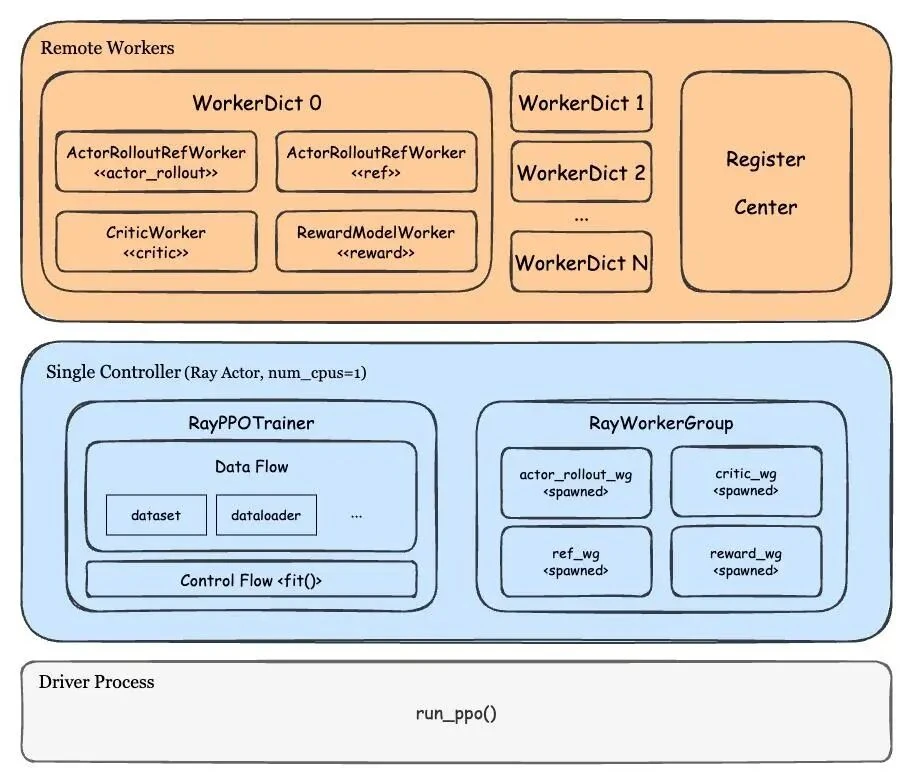
\includegraphics[width=0.8\textwidth]{HINH_VERL_ARCHITECTURE.png}
    \caption{Kiến trúc phân tán của Verl dựa trên nền tảng Ray.}
    \label{fig:verl_arch}
\end{figure}
% =========================================================================

Đặc biệt, để tối ưu hóa quá trình Rollout (giai đoạn mô hình tự sinh lời giải để lấy mẫu học tập), hệ thống tích hợp \textbf{vLLM} - một động cơ suy luận (inference engine) hiệu năng cao. Nhờ công nghệ PagedAttention cấp phát bộ nhớ động cho KV Cache, vLLM cho phép thực hiện Offline Batched Inference (sinh văn bản theo lô lớn) với tốc độ vượt trội, giải quyết triệt để nút thắt về thời gian sinh dữ liệu khổng lồ của các thuật toán RL (cơ chế này được minh họa ở Hình \ref{fig:paged_attention})\footnote{Nguồn tham khảo kiến trúc: \url{https://blog.vllm.ai/2023/06/20/vllm.html}}.

% =========================================================================
% TODO 5 (CHỖ NÀY NÊN CÓ ẢNH): Cơ chế PagedAttention hoặc Offline Batched Inference của vLLM.
% Nếu có ảnh, bạn tải vào thư mục và mở comment đoạn code dưới đây:

\begin{figure}[ht!]
    \centering
    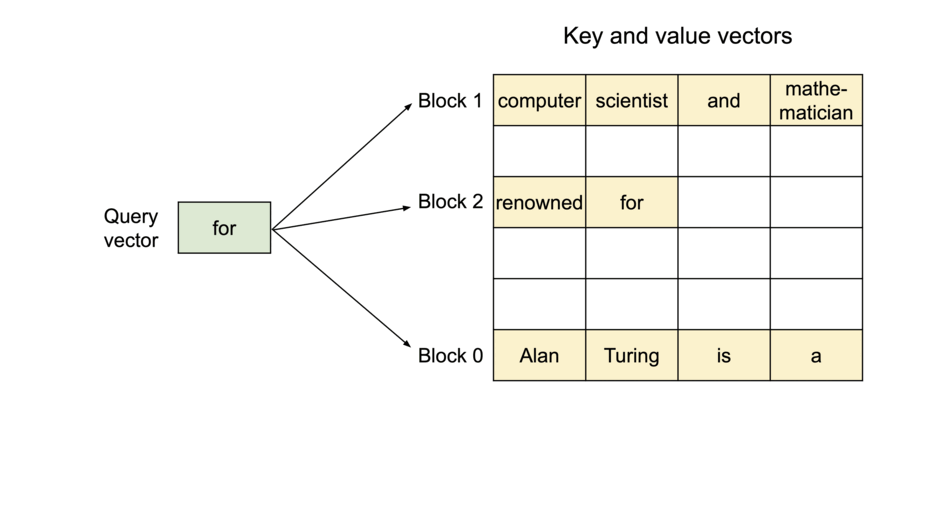
\includegraphics[width=0.8\textwidth]{HINH_PAGEDATTENTION.png}
    \caption{Cơ chế cấp phát bộ nhớ động PagedAttention của vLLM giúp tăng tốc độ sinh dữ liệu.}
    \label{fig:paged_attention}
\end{figure}
% =========================================================================

\chapter{PHƯƠNG PHÁP ĐỀ XUẤT VÀ THIẾT KẾ}

Chương này trình bày chi tiết về cải tiến cốt lõi của khóa luận đối với thuật toán SDPO: \textbf{Self-Distillation Policy Optimization kết hợp Cổng độ tin cậy (Reliability-Gated SDPO)}. Đây là phương pháp chủ đạo được áp dụng để giải quyết các thách thức đặc thù trong bài toán suy luận toán học.

\section{Giới hạn của SDPO truyền thống trong lĩnh vực Toán học}
Thuật toán SDPO nguyên bản (Vanilla SDPO) hoạt động dựa trên một giả định cốt lõi: mọi mục tiêu chưng cất (distillation targets) được tạo ra từ phản hồi (feedback-reprompted) đều có ích cho quá trình học tập. Giả định này có thể đúng trong một số tác vụ đơn giản, nhưng lại bộc lộ điểm yếu nghiêm trọng trong lĩnh vực toán học.

Trong giải toán, một câu trả lời sai không đơn thuần chỉ là kết quả sai, mà nó có thể bao gồm một chuỗi suy luận logic rất dài, trôi chảy nhưng chứa đựng các bước lập luận sai lầm (misleading reasoning). Việc SDPO truyền thống mù quáng ép mô hình học trò "bắt chước" (distill) những chuỗi suy luận kém chất lượng này sẽ vô tình củng cố tư duy sai lệch, dẫn đến hiện tượng triệt tiêu nhận thức và làm suy giảm năng lực tự khám phá của mô hình.

\section{Đề xuất SDPO kết hợp Cổng độ tin cậy (Reliability-Gated SDPO)}
Để khắc phục điểm yếu trên, phương pháp Reliability-Gated SDPO vẫn giữ nguyên cơ chế chưng cất tự thân của SDPO, nhưng can thiệp sâu vào khâu lựa chọn mục tiêu bằng một "Cổng độ tin cậy" (Reliability Gate) nhạy bén với phản hồi.

\subsection{Hàm mục tiêu (Objective Function)}
Giả sử $x_i$ là bài toán, $y_i$ là chuỗi câu trả lời của mô hình, $y_{i,<t}$ là các token đã sinh ra trước bước $t$. $f_i$ là tín hiệu phản hồi (kết hợp đúng/sai và lời giải mẫu nếu có). $\pi_\theta$ là chính sách hiện tại của mô hình.

Hàm mục tiêu của RL cơ bản (Base RL) chỉ tối ưu hóa dựa trên lợi thế:
\begin{equation}
    L_{base}(\theta) = L_{RL}(\pi_\theta)
\end{equation}

Thuật toán Vanilla SDPO nguyên bản bổ sung thêm một hàm mất mát chưng cất tự thân (tính bằng phân kỳ Kullback-Leibler - KL) áp dụng trên \textit{tất cả} các mục tiêu có sẵn:
\begin{equation}
    L_{vanilla}(\theta) = L_{RL}(\pi_\theta) + \lambda \times \mathbb{E}_{i,t} \left[ m_i \cdot \text{KL} \big( \pi_\theta(\cdot | x_i, y_{i,<t}) \| \text{stopgrad}(\pi_\theta(\cdot | x_i, f_i, y_{i,<t})) \big) \right]
\end{equation}

Phương pháp \textbf{Reliability-Gated SDPO} đề xuất thay đổi hàm mục tiêu bằng cách đưa vào hai biến số mới là \textbf{trọng số tín nhiệm} ($w_i$) và \textbf{cổng nhị phân} ($g_i$):
\begin{equation}
    L_{gate}(\theta) = L_{RL}(\pi_\theta) + \lambda \times \mathbb{E}_{i,t} \left[ m_i \cdot g_i \cdot w_i \cdot \text{KL} \big( \pi_\theta(\cdot | x_i, y_{i,<t}) \| \text{stopgrad}(\pi_\theta(\cdot | x_i, f_i, y_{i,<t})) \big) \right]
\end{equation}

\textbf{Giải thích chi tiết các thành phần trong công thức:}
\begin{itemize}
    \item $L_{gate}(\theta)$: Tổng hàm mục tiêu tối ưu hóa của hệ thống dựa trên bộ tham số $\theta$.
    \item $L_{RL}(\pi_\theta)$: Hàm mất mát của Học tăng cường (được tính dựa trên lợi thế GRPO/PPO để cực đại hóa phần thưởng).
    \item $\lambda$: Hệ số siêu tham số (hyperparameter) cân bằng mức độ ảnh hưởng của nhánh tự chưng cất so với nhánh RL gốc.
    \item $\mathbb{E}_{i,t}$: Kỳ vọng (giá trị trung bình) được tính toán trên toàn bộ các mẫu $i$ trong lô dữ liệu (batch) và từng token $t$ trong chuỗi.
    \item $m_i$: Mặt nạ mục tiêu gốc của SDPO ($m_i = 1$ nếu mục tiêu hợp lệ để chưng cất, $m_i = 0$ nếu bị cắt xén/vượt quá token).
    \item $g_i \in \{0, 1\}$: Cổng kiểm duyệt độ tin cậy. Chỉ mở ($g_i=1$) khi hệ thống tin tưởng độ an toàn của phản hồi $f_i$.
    \item $w_i \in [0, 1]$: Trọng số tín nhiệm (điều tiết lực chưng cất mạnh hay yếu tùy thuộc vào chất lượng của lời giải).
    \item $t$ và $y_{i,<t}$: $t$ là chỉ số của token hiện tại đang được sinh ra, còn $y_{i,<t}$ là toàn bộ các token đã sinh ra trước đó của câu trả lời $y_i$. Do mô hình ngôn ngữ sinh văn bản theo kiểu tự hồi quy (autoregressive), xác suất của token hiện tại luôn phụ thuộc vào câu hỏi và các token trước nó.
    \item $\pi_\theta(\cdot | x_i, y_{i,<t})$: Xác suất sinh token thứ $t$ của mô hình \textit{Student} (không được xem phản hồi).
    \item $\pi_\theta(\cdot | x_i, f_i, y_{i,<t})$: Xác suất sinh token thứ $t$ của mô hình \textit{Teacher} (chính là Student nhưng được cung cấp thêm thông tin $f_i$ để có "góc nhìn hồi tố").
    \item $\text{stopgrad}(\dots)$: Lệnh dừng lan truyền ngược (gradient), nhằm đóng băng các tham số của \textit{Teacher}, ép \textit{Student} phải học theo \textit{Teacher} chứ không phải ngược lại.
\end{itemize}
Trong đó, mô hình vẫn học hỏi từ phần thưởng RL, nhưng hàm mất mát tự chưng cất chỉ được kích hoạt ($g_i=1$) và nhận lực cập nhật tương ứng ($w_i$) đối với những mục tiêu thực sự đáng tin cậy.

\subsection{Cơ chế gán trọng số tín nhiệm (Reliability Weights)}
Hệ thống gán trọng số $w_i$ cho từng mục tiêu SDPO dựa trên phản hồi của hệ thống chấm điểm (math verifier), cụ thể như Bảng \ref{tab:reliability_weights}:

\begin{table}[ht!]
    \centering
    \begin{tabular}{|l|c|p{7.5cm}|}
        \hline
        \textbf{Trường hợp (Case)} & \textbf{Trọng số ($w_i$)} & \textbf{Ý nghĩa và Lý do} \\
        \hline
        Lời giải đúng đã xác minh & $1.0$ & Mục tiêu mạnh nhất; đã vượt qua hệ thống kiểm chứng phần thưởng. \\
        \hline
        Phản hồi tính đúng đắn an toàn & $0.4$ & Tín hiệu sửa lỗi hữu ích, nhưng không hoàn hảo như lời giải đã xác minh. \\
        \hline
        Phản hồi về định dạng & $0.2$ & Giúp ích cho định dạng, nhưng yếu về mặt chất lượng suy luận logic. \\
        \hline
        Đầu ra bị cắt xén (Truncated) & $0.0$ & Mục tiêu không an toàn; tuyệt đối không nên để mô hình bắt chước. \\
        \hline
        Không có lời giải \& phản hồi & $0.0$ & Không có mục tiêu SDPO nào hữu ích. \\
        \hline
    \end{tabular}
    \caption{Bảng phân bổ Trọng số tín nhiệm cho các mục tiêu SDPO.}
    \label{tab:reliability_weights}
\end{table}

\subsection{Cổng lọc và Ngân sách tính toán (Gate \& Batch Budget)}
Giá trị của cổng nhị phân $g_i$ được quyết định dựa trên một ngưỡng $\tau$ và ngân sách của một lô (batch budget) được định nghĩa qua tỷ lệ chọn tối đa (max selected fraction):
\begin{equation}
    g_i = \mathbf{1}[w_i \geq \tau] \land \text{selected\_by\_batch\_budget}(i)
\end{equation}
Với cấu hình mặc định, khóa luận thiết lập \textbf{$\tau = 0.4$} và \textbf{Tỷ lệ chọn tối đa $= 0.5$}. Điều này có nghĩa là Cổng lọc sẽ tự động từ chối hoàn toàn các mục tiêu thuần túy sửa lỗi định dạng ($w_i = 0.2$) và các mục tiêu bị cắt xén ($w_i = 0.0$). Ngay cả khi có rất nhiều mục tiêu vượt qua ngưỡng $\tau$, hệ thống cũng chỉ giữ lại tối đa $50\%$ số lượng mẫu có độ tin cậy cao nhất trong một lô để tiết kiệm tính toán.

\section{Các khía cạnh cải tiến đột phá}
Thuật toán Reliability-Gated SDPO mang lại hai sự cải tiến vượt bậc so với SDPO truyền thống:

\subsection{Nâng cao chất lượng mục tiêu (Higher-quality SDPO targets)}
Hàm mất mát SDPO giờ đây được tập trung hoàn toàn vào các mục tiêu đã được xác minh hoặc được dẫn xuất từ các phản hồi an toàn. Việc chủ động loại bỏ các mục tiêu có độ tin cậy thấp (những lời giải sai, nhiễu) giúp mô hình tránh khỏi việc mô phỏng các suy luận sai lệch, từ đó nâng cao chất lượng học tập và độ chính xác của mô hình khi giải quyết các bài toán hóc búa.

\subsection{Giảm thiểu chi phí tính toán (Lower SDPO compute)}
Đặc thù của thuật toán SDPO là tiêu tốn lượng tài nguyên khổng lồ do phải cộng dồn thêm các đầu vào của Teacher, tính toán logits của Teacher và cập nhật Actor. Bằng việc kết hợp thực thi mục tiêu thưa (sparse target execution), hệ thống bỏ qua toàn bộ việc tính toán hàm mất mát SDPO ở nhánh đắt đỏ cho các mẫu có độ tin cậy thấp. Điều này không chỉ bảo vệ mô hình khỏi dữ liệu rác mà còn giảm đáng kể thời gian và vRAM cần thiết cho quá trình huấn luyện.

% ------------------------- CHƯƠNG 4 -------------------------
\chapter{THỰC NGHIỆM VÀ ĐÁNH GIÁ}
\section{Môi trường và dữ liệu thực nghiệm}
\section{Thiết lập tham số huấn luyện}
\section{Kết quả thực nghiệm}
\section{Phân tích và đánh giá kết quả}

% ------------------------- CHƯƠNG 5 -------------------------
\chapter{KẾT LUẬN VÀ HƯỚNG PHÁT TRIỂN}
\section{Kết luận}
\section{Những đóng góp chính}
\section{Hướng phát triển tiếp theo}

% ------------------------- TÀI LIỆU THAM KHẢO -------------------------
\begin{thebibliography}{99}
\addcontentsline{toc}{chapter}{TÀI LIỆU THAM KHẢO}
\bibitem{hubotter2026sdpo}
Hübotter, J., Lübeck, F., Behric, L., Baumann, A., Bagatella, M., Marta, D., Hakimi, I., Shenfeld, I., Buening, T. K., Guestrin, C., \& Krause, A. \textit{Reinforcement Learning via Self-Distillation}. 2026.
\bibitem{kim2026degrade}
Kim, J., Luo, X., Kim, M., Lee, S., Kim, D., Jeon, J., Li, D., \& Yang, Y. \textit{Why Does Self-Distillation (Sometimes) Degrade the Reasoning Capability of LLMs?}. 2026.
\bibitem{kyars2026rlvr}
Kyars, K. \textit{Reinforcement Learning from Verifiable Rewards}. 2026.
\end{thebibliography}

\end{document}
